\documentclass[11pt]{beamer}
\usepackage{verbatim}
\usepackage{amsmath}
\usepackage{amsthm}
\usepackage{graphics}
\usepackage{multicol}
\usepackage{color}
\usepackage{stmaryrd}
\usefonttheme[onlymath]{serif}

\title{Progess Report 8}
\date{\today}
\author{Xie Li}
\begin{document}
\maketitle

\begin{frame}\frametitle{Overview of the Progress}
\begin{itemize}
\item After last survey of SV-COMP, implemented some utils help parse the information of SV-COMP cases.
\item Debugging the tool with Weizhi.
\item Other things...
\end{itemize}

\end{frame}


\begin{frame}\frametitle{Checking $\mathbf{G} (\neg \texttt{reachError()})$}

Since the uniqueness of function \texttt{reachError()}, checking can be done by

\begin{itemize}
\item Sample the paths from automaton. Sampler return the path once \texttt{reachError()} is met.

\item Check the feasibility of the \texttt{reachError()} path.
\end{itemize}
\end{frame}

\begin{frame}\frametitle{Parsing}
\begin{center}
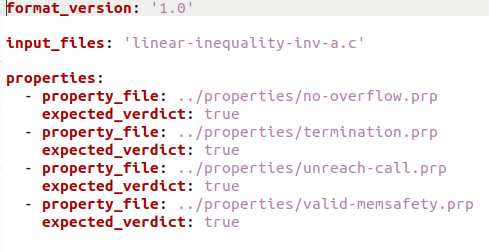
\includegraphics[scale=0.4]{yaml.png}
\end{center}
Use C++ tool: yaml-cpp to do the parsing and extract:
\begin{itemize}
\item path of input file
\item path of property file
\item expected verdict 
\end{itemize}
\end{frame}
\begin{frame}\frametitle{Current Problem Encountered}
\textbf{Interprocedural Analysis}
\begin{itemize}
\item \texttt{void checkAssertion(bool condition)}

\item In the translation, for every function we construct an automaton for the function. 

\item When sampling the path in the automaton.
Merge the automaton of called procedure into the main automaton?


\end{itemize}

\end{frame}

\begin{frame}\frametitle{Checking Path Feasibility}

After converting the CFG to an automaton e.g. DFA. We are able to sample a path of the automaton and do the path feasibility checking.
 
Current path feasibility check:
\begin{itemize}
\item Frontend: C$\rightarrow$ IR $\rightarrow$ CFG.
\item Modelling: CFG$\rightarrow$ DFA, where alphabet of DFA is the set of instructions.

\item Sampling a path and conjuncts condition induced by the instructions result in the path condition.
\end{itemize}

We are now able to generate path conditions for programs with only arithmetic operations. 
\end{frame}

\begin{frame}\frametitle{Checking LTL Formula on a Path}
Beyond the path condition, we can also check LTL property on a path. 
\end{frame}

\end{document}